\documentclass[11pt, hyperref={urlcolor=red,% Liens vers une page web
            linkcolor=blue, %Liens internes au document
            colorlinks=true}]{beamer}  
            
\usetheme{Warsaw} 

%thèmes prédéfinis de Beamer 
%Antibes, boxes, classic, Darmstadt, Madrid
% Montpellier, Warsaw, Bergen, Berkeley, Goettingen, sidebar


%%%%%%%Tit\title{Titre principal}

\title[int\'egration]{Exemples du cours du chapitre calcul int\'egral 2019/2020}
%\subtitle{Sous titre}
\author[F.Junier]{Fr\'ed\'eric Junier}
\institute[Le Parc]{{\centering Lyc\'ee du Parc \\
1 Boulevard Anatole France \\ 69006 Lyon }}
\date[\today]{\today}

\usepackage{etex}

%%%%%%%%%%%%Encodage du fichier source %%%%%%%%%%%
\usepackage[T1]{fontenc}
\usepackage[utf8]{inputenc}

\usepackage{lmodern}
\usepackage{url}
\usepackage[np]{numprint}


%%%%%%%%%%%%Là encore il y a de grosses différences entre le monde anglo-saxon et les francophones.Le séparateur des décimales est un point en anglais et une virgule en français. Leséparateur des milliers est une virgule en anglais et une espace insécable en français. Ilest préférable d’utiliser le package numprint (\usepackage{numprint}) qui associé àfrenchb produira la bonne typographie.
%123456789 = 123456789 \numprint{123456789} = 123 456 789  \numprint{3,1415926535897932384626} = 3,141 592 653 589 793 238 462 6  \numprint{12.34} = 12,34  En plus tu peux préciser les unités de cette façon : \numprint[kg]{12.34} = 12,34 kg ou encore \numprint[\degres C]{22} = 22°C Si tu veux utiliser le raccourci \np{} au lieu de \numprint{}, il te faut charger le package de cette façon : \usepackage[np]{numprint}


%%%%%%%%%%PSTricks%%%%%%%%%%%%

\usepackage{pstricks,pst-plot,pst-text,pst-tree,pst-eps,pst-fill,pst-node,pst-math,pstricks-add,pst-xkey,pst-eucl}


%%%%%%%Tikz%%%%%%%%%%%%%%%
\usepackage{pgf,tikz,tkz-tab}
% Pour les tableaux de signes ou de variations avec tkz-tab voir https://zestedesavoir.com/tutoriels/439/des-tableaux-de-variations-et-de-signes-avec-latex/#1-13389_tikz-un-package-qui-en-a-dans-le-ventre
\usetikzlibrary{arrows}
\usetikzlibrary{shapes.geometric}
\usetikzlibrary{shapes.geometric}
\usetikzlibrary{petri}
\usetikzlibrary{decorations}
\usetikzlibrary{arrows}
\usetikzlibrary{math}
 %Variables must be declared in a tikzmath environment but
       % can be used outside
%       \tikzmath{int \n; \n = 508; \x1 = 1; \y1 =1; 
%                   %computations are also possible
%                    \x2 = \x1 + 1; \y2 =\y1 +3; } 


%%%%%%%%%%%%%%%%%%%%%%%%%%%%%%%%%%%%%%%%
%%%%%%%%%%%Commandes Tikz Perso%%%%%%%%%%%%%%%

% Définition des nouvelles options xmin, xmax, ymin, ymax
% Valeurs par défaut : -3, 3, -3, 3
\tikzset{
xmin/.store in=\xmin, xmin/.default=-3, xmin=-3,
xmax/.store in=\xmax, xmax/.default=3, xmax=3,
ymin/.store in=\ymin, ymin/.default=-3, ymin=-3,
ymax/.store in=\ymax, ymax/.default=3, ymax=3,
}
% Commande qui trace la grille entre (xmin,ymin) et (xmax,ymax)
\newcommand {\grille}[2]
{\draw[help lines,black, thick] (\xmin,\ymin) grid[xstep=#1, ystep=#2] (\xmax,\ymax);}
% Commande \axes
\newcommand {\axes} {
\draw[->,very thick] (\xmin,0) -- (\xmax,0);
\draw[->,very thick] (0,\ymin) -- (0,\ymax);
\draw (0.95*\xmax, 0) node[above] {$x$};
\draw (0, 0.95*\ymax) node[left] {$y$};
}
% Commande qui limite l?affichage à (xmin,ymin) et (xmax,ymax)
\newcommand {\fenetre}
{\clip (\xmin,\ymin) rectangle (\xmax,\ymax);}

%Exemple d'utilisation

%\begin{center}
%\begin{tikzpicture} [xmin=-2,xmax=2,ymin=0,ymax=5]
%\grille{1} \axes \fenetre
%\draw plot[smooth] (\x,\x^2);
%\end{tikzpicture}
%\end{center}

%style pour la perspective cavalière française
%voir Tikz pour l'impatient page 68
\tikzset{math3d/.style=
{x= {(-0.353cm,-0.353cm)}, z={(0cm,1cm)},y={(1cm,0cm)}}}

%%%%%%%Symbole pour code calculatrice%%%%%%

%Flèche remplie pour défilement de menu

\newcommand{\flechefillright}{
\begin{tikzpicture}[scale=0.15] \fill (0,0)--(2,1)--(0,2)--cycle;
\end{tikzpicture}}

%%%%%%%%%%%%%Symboles pour calculatrice Casio%%%%
\newcommand{\execasio}{\Pisymbol{psy}{191}} %Retour chariot
\newcommand{\dispcasio}{\begin{pspicture}(.1,.1)\pspolygon*(.1,0)(.1,.1)\end{pspicture}} %Triangle « Disp »
\newcommand{\dispcasiotikz}{\begin{tikzpicture}[scale=0.2]
\fill (0,0) -- (1,0) -- (1,1) -- cycle;
\end{tikzpicture}} %Triangle « Disp »
%


%%%%%%%%%%%%%%%%%%%Présentation de codes sources%%%%%%%%%%%%%%%%%
\usepackage{listings}
%On utilise l?environnement lstlisting pour insérer
%un code source.
%En plus de l?environnement lstlisting, on peut également utiliser la
%commande \lstinline qui fonctionne comme la commande \verb, en ce
%sens qu?on peut utiliser n?importe quel caractère comme délimiteur. Enfin,
%la commande \lstinputlisting permet de charger un code source depuis
%un fichier externe.
%Il y a deux manières de préciser des options : soit via l?option de l?envi-
%ronnement ou de la commande, soit en utilisant la commande \lstset
%qui permet de définir des options de manière globale.

\lstset{ %
  language=Python,                % the language of the code
  basicstyle=\ttfamily,           % the size of the fonts that are used for the code
  %numbers=left,                   % where to put the line-numbers
  numberstyle=\tiny,  % the style that is used for the line-numbers
  %stepnumber=2,                   % the step between two line-numbers. If it's 1, each line 
                                  % will be numbered
  %numbersep=5pt,                  % how far the line-numbers are from the code
  backgroundcolor=\color{white},      % choose the background color. You must add \usepackage{color}
  showspaces=false,               % show spaces adding particular underscores
  showstringspaces=false,         % underline spaces within strings
  showtabs=false,                 % show tabs within strings adding particular underscores
  frame=single,                   % adds a frame around the code
  rulecolor=\color{black},        % if not set, the frame-color may be changed on line-breaks within not-black text (e.g. comments (green here))
  tabsize=4,                      % sets default tabsize to 2 spaces
  captionpos=b,                   % sets the caption-position to bottom
  breaklines=true,                % sets automatic line breaking
  breakatwhitespace=false,        % sets if automatic breaks should only happen at whitespace
  %title=\lstname,                   % show the filename of files included with \lstinputlisting;
                                  % also try caption instead of title
  breakindent=1cm,
  keywordstyle=\color{blue},          % keyword style
  commentstyle=\color{red},       % comment style
  %stringstyle=\ttfamily\color{green},         % string literal style
  escapeinside={\%*}{*)},            % if you want to add LaTeX within your code
  morekeywords={*,...},              % if you want to add more keywords to the set
  deletekeywords={...}              % if you want to delete keywords from the given language
  upquote=true,columns=flexible,
xleftmargin=1cm,xrightmargin=1cm,
 inputencoding=utf8,			%Les lignes qui suivent sont pour le codage utf8
  extendedchars=true,
  literate=%
            {é}{{\'{e}}}1
            {è}{{\`{e}}}1
            {ê}{{\^{e}}}1
            {ë}{{\¨{e}}}1
            {û}{{\^{u}}}1
            {ù}{{\`{u}}}1
            {â}{{\^{a}}}1
            {à}{{\`{a} }}1
            {î}{{\^{i}}}1
            {ô}{{\^{o}}}1
            {ç}{{\c{c}}}1
            {Ç}{{\c{C}}}1
            {É}{{\'{E}}}1
            {Ê}{{\^{E}}}1
            {À}{{\`{A}}}1
            {Â}{{\^{A}}}1
            {Î}{{\^{I}}}1
}

\lstdefinestyle{rond}{
  numbers=none,
  frameround =tttt
}

\lstdefinestyle{compil}{
  numbers=none,
  backgroundcolor=\color{gristclair}
}
%\lstset{language=Python,basicstyle=\small , frame=single,tabsize=4,showspaces=false,showtabs=false,showstringspaces=false,numbers=left,numberstyle=\tiny , extendedchars=true}

%%%%%%%%%%%AmsMaths%%%%%%
\usepackage{amsmath,amsfonts,amssymb}
\usepackage{pifont,fourier}
\usepackage{ bclogo}


%%%%%Commande \DeclareMathOperator pour définir de nouveaux opérateurs (en lettres romaines droites)%%%%%
%\DeclareMathOperator{\sh}{sh}
%\DeclareMathOperator{\ch}{ch}

%%%%%%%%%%%%%%%%%%Maths divers%%%%%%%%%%%%%%%%%%%%%%%%%
%Delimiteurs
\newcommand{\delim}[3]{\raise #1\hbox{$\left #2\vbox to #3{}\right.$}}


%%%%%%%%%%%%%Nombres%%%%%%%%%%%%%%%%

%Ensemble prive de...
%\newcommand{\prive}{\boi}%{\backslash}

%Ensembles de nombres%%%%%%%%%%%%%%%%%
\newcommand{\R}{\mathbb{R}}
\newcommand{\N}{\mathbb{N}}
\newcommand{\D}{\mathbb{D}}
\newcommand{\Z}{\mathbb{Z}}
\newcommand{\Q}{\mathbb{Q}}
\newcommand{\C}{\mathbb{C}}
\newcommand{\df}{~\ensuremath{]0;+\infty[}~}
\newcommand{\K}{\mathbb{K}}

%%%%%%%%Arithmetique%%%%%%%%%%
%PGCD, PPCM
\newcommand{\PGCD}{\mathop{\rm PGCD}\nolimits}
\newcommand{\PPCM}{\mathop{\rm PPCM}\nolimits}

%Intervalles
\newcommand{\interoo}[2]{]#1\, ;\, #2[}
\newcommand{\Interoo}[2]{\left]#1\, ;\, #2\right[}
\newcommand{\interof}[2]{]#1\, ;\, #2]}
\newcommand{\Interof}[2]{\left]#1\, ;\, #2\right]}
\newcommand{\interfo}[2]{[#1\, ;\, #2[}
\newcommand{\Interfo}[2]{\left[#1\, ;\, #2\right[}
\newcommand{\interff}[2]{[#1\, ;\, #2]}
\newcommand{\Interff}[2]{\left[#1\, ;\, #2\right]}
%\newcommand\interentiers #1#2{[\! [#1\, ;\, #2]\! ]}
\newcommand{\interentiers}[2]{\llbracket #1\, ;\, #2\rrbracket}
%


%%%%%%%%%%%%%%Nombres complexes%%%%%

\newcommand{\ic}{\text{i}}
%\newcommand{\I}{\text{i}}
\newcommand{\im}[1]{\text{Im}\left(#1\right)}
\newcommand{\re}[1]{\text{Re}\left(#1\right)}
\newcommand{\Arg}[1]{\text{arg}\left(#1\right)}
\newcommand{\Mod}[1]{\left[#1\right]}
%Parties entière, réelle, imaginaire, nombre i
\newcommand{\ent}[1]{\text{E}\left(#1\right)}
\renewcommand{\Re}{\mathop{\rm Re}\nolimits}
\renewcommand{\Im}{\mathop{\rm Im}\nolimits}
\renewcommand{\i}{\textrm{i}}

%%%%%%%%%%%Probabilites et statistiques%%%%%
\newcommand{\loibinom}[2]{\mathcal{B}\left(#1\ ; \ #2 \right)}
\newcommand{\loinorm}[2]{\mathcal{N}\left(#1\ ; \ #2 \right)}
\newcommand{\loiexp}[1]{\mathcal{E}\left(#1\right)}
\newcommand{\proba}[1]{\mathbb{P}\big(#1\big)}
\newcommand{\probacond}[2]{\mathbb{P}_{#2}\big(#1\big)}
\newcommand{\esperance}[1]{\mathbb{E}\left(#1\right)}
\newcommand{\variance}[1]{\mathbb{V}\left(#1\right)}
\newcommand{\ecart}[1]{\sigma\left(#1\right)}
\newcommand{\dnormx}{\frac{1}{\sqrt{2\pi}} \text{e}^{-\frac{x^2}{2}}}
\newcommand{\dnormt}{\frac{1}{\sqrt{2\pi}} \text{e}^{-\frac{t^2}{2}}}
\newcommand{\nbalea}[2]{\reinitrand[first=#1, last=#2, counter=num]  \rand $\thenum$}  %retourne un entier aleatoire antre les bornes #1 et #2 comprises
%Covariance
\newcommand{\cov}{\mathop{\rm cov}\nolimits}
%


%%%%%%%%%%Analyse%%%%%%%%%%%

%%%%%%%%%%%Courbe%%%%%%%%%%%%
\newcommand{\courbe}[1]{\ensuremath{\mathcal{C}_{#1}}}

%%%%%%%Fonction exponentielle%%%%%
\newcommand{\fe}{~fonction exponentielle~}
\newcommand{\e}{\text{e}}

%Fonction cotangente
\newcommand{\cotan}{\mathop{\rm cotan}\nolimits}
%%%%%%%%%%%%%%%%%%%%%%%%%%%%%%%%%%%%%%%%%
%
%Fonctions hyperboliques
\newcommand{\ch}{\mathop{\rm ch}\nolimits}
\newcommand{\sh}{\mathop{\rm sh}\nolimits}


%%%%%%%%%%%%%%Limites%%%%%%
\newcommand{\limite}[2]{\lim\limits
_{x \to #1} #2}
\newcommand{\limitesuite}[1]{\lim\limits
_{n \to +\infty} #1}
\newcommand{\limiteg}[2]{\lim\limits
_{\substack{x \to #1 \\ x < #1 }} #2}
\newcommand{\limited}[2]{\lim\limits
_{\substack{x \to #1 \\ x > #1 }} #2}

%%%%%%%%%%Continuité%%%%%%%%%%%
\newcommand{\TVI}{théorème des valeurs intermédiaires}

%%%%%%%%%%%Suites%%%%%%%%%%%%
\newcommand{\suite}[1]{\ensuremath{\left(#1_{n}\right)}}
\newcommand{\Suite}[2]{\ensuremath{\left(#1\right)_{#2}}}
%

%%%%%%%%%%%%%%%Calcul intégral%%%%%%
\newcommand{\dx}{\ensuremath{\text{d}x}}		% dx
\newcommand{\dt}{\ensuremath{\text{d}t}}		% dt
\newcommand{\du}{\ensuremath{\text{d}u}}		% dx
\newcommand{\dtheta}{\ensuremath{\text{d}\theta}}		% dtheta
\newcommand{\dy}{\ensuremath{\text{d}y}}		% dy
\newcommand{\dq}{\ensuremath{\text{d}q}}		% dq

%%%Intégrale%%%
\newcommand{\integralex}[3]{\int_{#1}^{#2} #3 \ \dx}
\newcommand{\integraleu}[3]{\int_{#1}^{#2} #3 \ \du}
\newcommand{\integralet}[3]{\int_{#1}^{#2} #3 \ \dt}
\newcommand{\integraletheta}[3]{\int_{#1}^{#2} #3 \ \dtheta}

%%%%%Equivalent%%
\newcommand{\equivalent}[1]{\build\sim_{#1}^{}}

%o et O%%%%
\renewcommand{\o}[2]{\build o_{#1\to #2}^{}}
\renewcommand{\O}[2]{\build O_{#1\to #2}^{}}



%%%%%%%%%%%%%%%Geometrie%%%%%%%%%%%%%%%%%%%%%%%

%%%%%%%%%%%%%%%Reperes%%%%%%%%%%%%%%
\def\Oij{\ensuremath{\left(\text{O},~\vect{\imath},~\vect{\jmath}\right)}}
\def\Oijk{\ensuremath{\left(\text{O},~\vect{\imath},~ \vect{\jmath},~ \vect{k}\right)}}
\def\Ouv{\ensuremath{\left(\text{O},~\vect{u},~\vect{v}\right)}}
\renewcommand{\ij}{(\vec\imath\, ;\vec\jmath\,)}
\newcommand{\ijk}{(\vec\imath\, ;\vec\jmath\, ;\vec k\,)}
\newcommand{\OIJ}{(O\,;\, I\,;\, J\,)}
\newcommand{\repere}[3]{\big(#1\, ;\,\vect{#2} ;\vect{#3}\big)}
\newcommand{\reperesp}[4]{\big(#1\, ;\,\vect{#2} ;\vect{#3} ;\vect{#4}\big)}

%%%%%%%%%Coordonnees%%%%%%%%%%%%%%
\newcommand{\coord}[2]{(#1\, ;\, #2)}
\newcommand{\bigcoord}[2]{\big(#1\, ;\, #2\big)}
\newcommand{\Coord}[2]{\left(#1\, ;\, #2\right)}
\newcommand{\coordesp}[3]{(#1\, ;\, #2\, ;\, #3)}
\newcommand{\bigcoordesp}[3]{\big(#1\, ;\, #2\, ;\, #3\big)}
\newcommand{\Coordesp}[3]{\left(#1\, ;\, #2\, ;\, #3\right)}
\newcommand{\Vcoord}[3]{\begin{pmatrix} #1 \\ #2 \\ #3 \end{pmatrix}}
%Symboles entre droites
%\newcommand{\paral}{\sslash}
\newcommand{\paral}{\mathop{/\!\! /}}
%

%%%%%%%%%Produit scalaire, Angles%%%%%%%%%%
\newcommand{\scal}[2]{\vect{#1} \, \cdot \, \vect{#2}}
\newcommand{\Angle}[2]{\left(\vect{#1} \, , \, \vect{#2}\right)}
\newcommand{\Anglegeo}[2]{\left(\widehat{\vect{#1} \, ; \, \vect{#2}}\right)}
\renewcommand{\angle}[1]{\widehat{#1}}
\newcommand{\anglevec}[2]{\left(\vect {#1}\, ,\,\vect {#2} \right)}
\newcommand{\anglevecteur}[2]{(#1\, , \, #2)}
\newcommand{\Anglevec}[2]{(\vecteur{#1}\, ,\,\vecteur{#2})}
\newcommand{\prodscal}[2]{#1 \, \cdot \, #2}
%


%Arc
%\newcommand{\arc}[1]{\wideparen{#1}}
\newcommand{\arcoriente}[1]{\overset{\curvearrowright}{#1}}
%
%


%%%%%%%%%%%%%%%Normes%%%%%%%%%%%%%%%%
\newcommand{\norme}[1]{\left\| #1\right\|}
\newcommand{\normebis}[1]{\delim{2pt}{\|}{9pt}\! #1\delim{2pt}{\|}{9pt}}
\newcommand{\normetriple}[1]{\left |\kern -.07em\left\| #1\right |\kern -.07em\right\|}
\newcommand{\valabs}[1]{\big| \, #1 \, \big|}
%

%%%%%%%%%%%%%%%%%%%%%%%%%%%Degré%%%%%%
%\newcommand{\Degre}{\ensuremath{^\circ}}
%La commande \degre est déjà définie dans le package babel

%%%%%%%%%%Vecteurs%%%%%%%%%%%
\newcommand{\vect}[1]{\mathchoice%
{\overrightarrow{\displaystyle\mathstrut#1\,\,}}%
{\overrightarrow{\textstyle\mathstrut#1\,\,}}%
{\overrightarrow{\scriptstyle\mathstrut#1\,\,}}%
{\overrightarrow{\scriptscriptstyle\mathstrut#1\,\,}}}



%%%%%%%%%%%%%Algebre%%%%%%%%%%%%%%%


%%%%%%%%%%Systemes%%%%%%%%%%%
%Systemes
\newcommand{\sys}[2]{
\left\lbrace
 \begin{array}{l}
  \negthickspace\negthickspace #1\\
  \negthickspace\negthickspace #2\\
 \end{array}
\right.\negthickspace\negthickspace}
\newcommand{\Sys}[3]{
\left\lbrace
 \begin{array}{l}
  #1\\
  #2\\
  #3\\
 \end{array}
\right.}
\newcommand{\Sysq}[4]{
\left\lbrace
 \begin{array}{l}
  #1\\
  #2\\
  #3\\
  #4\\
 \end{array}
\right.}
%
%

%%%%%%%%%%%%%%%%Matrices%%%%%%%%%%%%%%%%%%
%Comatrice
\newcommand{\com}{\mathop{\rm com}\nolimits}
%
%
%Trace
\newcommand{\tr}{\mathop{\rm tr}\nolimits}
%
%
%Transposee
\newcommand{\transposee}[1]{{\vphantom{#1}}^t\negmedspace #1}
%
%
%Noyau
\newcommand{\Ker}{\mathop{\rm Ker}\nolimits}
%
%

%
%Matrices
\newcommand{\Mn}{\mathcal M_n}
\newcommand{\matrice}[4]{
\left(
 \begin{array}{cc}
  #1 & #2 \\
  #3 & #4
 \end{array}
\right)}

\newcommand{\Matrice}[9]{
\left(
 \begin{array}{ccc}
  #1 & #2 & #3\\
  #4 & #5 & #6\\
  #7 & #8 & #9
 \end{array}
\right)}
\newcommand{\Vect}[3]{
\left(\negmedspace
 \begin{array}{c}
  #1\\
  #2\\
  #3
 \end{array}\negmedspace
\right)}
\newcommand{\Ideux}{\matrice{1}{0}{0}{1}}
\newcommand{\Itrois}{\Matrice{1}{0}{0}{0}{1}{0}{0}{0}{1}}
%
%
%Determinants
\newcommand{\determinant}[4]{
\left|
 \begin{array}{cc}
  #1 & #2 \\
  #3 & #4
 \end{array}
\right|}
\newcommand{\Determinant}[9]{
\left|
 \begin{array}{ccc}
  #1 & #2 & #3\\
  #4 & #5 & #6\\
  #7 & #8 & #9
 \end{array}
\right|}

%%%%%%%%%%%%%%Calculs en Latex%%%%%%%%%%%%%

\usepackage[first=1,last=100]{lcg}  %%%%%%%générer des nombres pseudo aléatoires
%%%%
\usepackage{calc} %   pour faire des calculs%%


%%%%Mise en page%%%%%
\usepackage{fancybox}
\usepackage{lastpage}
\usepackage{hyperref}
%À mettre dans le préambule pour faire apparaitre le plan à chaque section 

\AtBeginSection[ ]
{
\begin{frame}<beamer>
\frametitle{Plan}
\tableofcontents[currentsection]
\end{frame}
}

%%%%%%%¨Puces%%%%%%%%%%%%
\usepackage{enumerate}


%%%%%%%%%%%%Graphiques%%%%%%%%%%%%%%
\usepackage{graphicx,pgf}				
\usepackage{pstricks,pst-plot,pst-text,pst-tree,pst-eps,pst-node,pst-math,pstricks-add}
 


%%%%%%Numérotation des automatismes%%%%%%
\newcounter{autocompteur}
\setcounter{autocompteur}{0}
\newcommand{\automatisme}[1]{\addtocounter{autocompteur}{1}\frametitle{Automatisme  \theautocompteur  \textit{ thème : #1}}}
%%%%%%%%%%%%%%%%%%%%%%%%%%%%%%%%%%%%%%%%%%%%%%%%

%%%%%%%%%%%%%%%Francisation%%%%%%%%%%%%%%
\usepackage[french]{babel}
\frenchbsetup{StandardLists=true}

%%%%%%%%%%%%%%%%%%%%%%%%%%%%%%%%%%%%%%%%%



\begin{document}

\frame{\titlepage}




\begin{frame}
\frametitle{Table des matières}
\begin{itemize}
	\item \hyperlink{exemple1}{Exemple 1}
	\item \hyperlink{exemple2}{Exemple 2}
	\item \hyperlink{exemple3}{Exemple 3}
	\item \hyperlink{exemple4}{Exemple 4}
	\item \hyperlink{exemple5}{Exemple 5}
	\item \hyperlink{exemple6}{Exemple 6}
		\item \hyperlink{exemple7}{Exemple 7}
			\item \hyperlink{exemple8}{Exemple 8}
			\item \hyperlink{exemple9}{Exemple 9}
				\item \hyperlink{exemple10}{Exemple 10}
						\item \hyperlink{exemple11}{Exemple 11}
						\item \hyperlink{exemple12}{Exemple 12}
						\item \hyperlink{exemple13}{Exemple 13}
						\item \hyperlink{exemple14}{Exemple 14}
						\item \hyperlink{exemple15}{Exemple 15}
						\item \hyperlink{exemple16}{Exemple 16}
\end{itemize}

\end{frame}

\begin{frame}
\frametitle{Exemple 1 Partie 1}
\label{exemple1}

Soit $f$ la fonction définie sur $\Interff{0}{2}$ par $f(x)=2-x$.

La surface dont l'aire est égale à  intégrale  $I=\integralex{1}{2}{f(x)}$ est le triangle $BCD$  rectangle isocèle en $C$  dont l'aire est $\frac{1}{2} \times 1 \times 1=\frac{1}{2}$.

\begin{center}
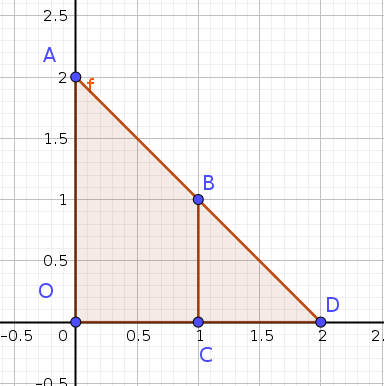
\includegraphics[scale=0.4]{images/exemple1.png}
\end{center}

\end{frame}

\begin{frame}
\frametitle{Exemple 1 Partie 2}
Soit $f$ la fonction définie sur $\Interff{0}{2}$ par $f(x)=2-x$.

La surface dont l'aire est égale à  intégrale  $I=\integralex{0}{1}{f(x)}$ est le trapèze $OABC$  rectangle isocèle en $O$  dont l'aire est $\frac{1}{2} \times ( OA + BC) \times OC = \frac{3}{2}$.

\begin{center}
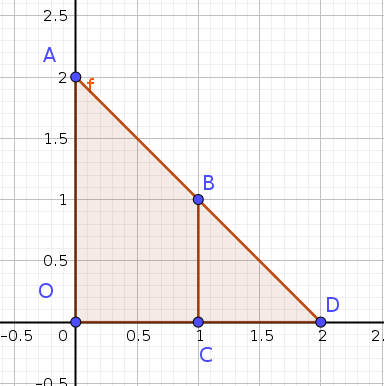
\includegraphics[scale=0.4]{images/exemple1.png}
\end{center}

\end{frame}


\begin{frame}
\frametitle{Exemple 2 Question 1}
\label{exemple2}

Soit $M(t)$ un point mobile sur un axe tel que à chaque instant $t \in \Interfo{0}{+\infty}$ (en secondes)  on conna\^it sa vitesse instantanée $v(t)$ en mètres par seconde. 

A l'instant $t=0$, le point mobile est à l'origine de l'axe  et pour tout $t \in \Interfo{0}{+\infty}$, on a $v(t)=3 \ \text{m}.\text{s}^{-1}$.

\begin{itemize}

\item \textbf{Question 1}  La fonction $v$ est constante donc dérivable donc continue sur $\Interfo{0}{+\infty}$.

$\int_{0}^{4}v(t)\dt$  est l'aire du rectangle $EFGH$ c'est-à-dire $4 \times 3 = 12$.

On peut l'interpréter comme la distance parcourue par le mobile en $3$ secondes. Notons que la dimension de l'intégrale est celle de $v(t)\dt$ : vitesse $\times$ temps = distance.
\end{itemize}

\begin{center}
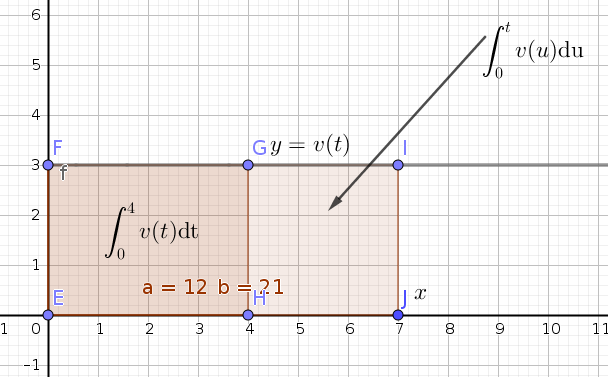
\includegraphics[scale=0.2]{images/exemple2.png}
\end{center}

\end{frame}



\begin{frame}
\frametitle{Exemple 2 Question 2}


\begin{itemize}

\item \textbf{Question 2}  $\int_{2}^{5}v(t)\dt$ est égale à $(5 - 2) \times 3 = 9$. C'est la distance parcourue par le mobile entre les instants $t=2$ et $t=5$ à une vitesse de $3$ m.s$^{-1}$. $\frac{1}{5-2}\int_{2}^{5}v(t)\dt$ est égale à $\frac{\text{distance}}{\text{temps}}=\frac{9}{3}$, c'est la vitesse moyenne du mobile entre les instants $t=2$ et $t=5$. Comme sa vitesse est constante, c'est sa vitesse instantanée à tout instant. On a un exemple, d'utilisation de l'intégrale dans un calcul de valeur moyenne. Notons que $\frac{1}{5-2}\int_{2}^{5}v(t)\dt$ a la même dimension que $v(t)$, c'est une vitesse.
\end{itemize}



\end{frame}



\begin{frame}
\frametitle{Exemple 2 Question 3}


\begin{itemize}

\item \textbf{Question 3}  $g(t)=\integraleu{0}{t}{v(u)}$ est l'aire du rectangle $EFIJ$ c'est-à-dire $t \times 3 = 3t$.

On peut l'interpréter comme la distance parcourue par le mobile en $t3$ secondes. 

$g$ est une fonction linéaire donc elle est dérivable sur $\Interfo{0}{+\infty}$ et $g'(t)=3$.  On remarque que $g'(t)=v(t)$. On peut l'expliquer en prenant  la limite du taux de variation  $\frac{g(t+h)-g(t)}{h} = \frac{3(t+h)-3t}{h}=3$ quand $h$ tend vers $0$.

 $g(t)=\integraleu{0}{t}{v(u)}$ est une primitive de $v$.

\begin{center}
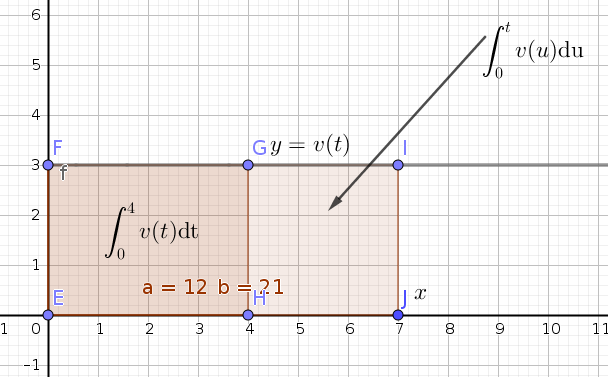
\includegraphics[scale=0.2]{images/exemple2.png}
\end{center}


\end{itemize}



\end{frame}




\begin{frame}
\frametitle{Exemple 3}

Voir \href{https://mybinder.org/v2/gh/frederic-junier/TS-2019-2020/master?filepath=CalculIntegral/ressources/Cours_Calcul_Integral_2020_Eleve.ipynb}{Notebook} et  \href{https://frederic-junier.github.io/TS-2019-2020/CalculIntegral/ressources/Cours_Calcul_Integral_2020_Eleve-Corrige.pdf}{Corrigé} (suivez les liens).


\end{frame}



\begin{frame}
\frametitle{Exemple 4 Question 1}

Soit $f$ définie sur $\Interfo{0}{+\infty}$ par $f(t)=\frac{1}{\sqrt{2\pi}}\text{e}^{-\frac{t^2}{2}}$.

\begin{itemize}

\item $f$ est dérivable sur  $\Interfo{0}{+\infty}$ et $f'(t)=\frac{1}{\sqrt{2\pi}} \times (-t)\text{e}^{-\frac{t^2}{2}}$. Pour  tout réel $t<0$, on a $f'(t)>0$ et $f'(0)=0$.

On en déduit que $f$ est  strictement décroissante sur $\Interoo{0}{+\infty}$.

Puisque $\lim\limits_{x \to -\infty} \text{e}^{x}=0$, on a par composition $\lim\limits_{t \to +\infty} \text{e}^{-\frac{t^2}{2}}=0$.

%Puisque pour tout réel $t$, on a $f(t)=f(-t)$, $f$ est paire et donc $\lim\limits_{t \to +\infty} f(t)=\lim\limits_{t \to -\infty} f(t)=0$.

\end{itemize}


\end{frame}



\begin{frame}
\frametitle{Exemple 4 Questions 2 et 3}

$f$ est dérivable donc continue  sur $\Interfo{0}{+\infty}$.

De plus, pour tout $t \geqslant 0$, on a  $f(t)=\frac{1}{\sqrt{2\pi}}\text{e}^{-\frac{t^2}{2}}$ donc $f(t) \geqslant 0$.

On peut appliquer le théorème fondamental, qui nous permet d'affirmer que  $F:x \mapsto \integralet{0}{x}{f(t)}$ est définie et dérivable sur $\Interfo{0}{+\infty}$  et que pour tout réel $x \geqslant 0$, $F'(x)=f(x)$.

Notez qu'on utilise plutôt $x$ pour $F$ et $t$ pour $F'=f$ mais qu'on pourrait écrire : pour tout réel $t \geqslant 0$, $F'(t)=f(t)$.

Puisque $f$ est strictement positive sur $\Interoo{0}{+\infty}$ et ne s'annule qu'en 0, on en déduit que $F$ est strictement croissante sur $\Interfo{0}{+\infty}$. Page suivante un graphique qui permet de comprendre pourquoi $F(x)$ aire sous la courbe de $f$ entre $0$ et $x$ est croissante.


\end{frame}



\begin{frame}
\frametitle{Exemple 4 Questions 2 et 3}

\begin{center}
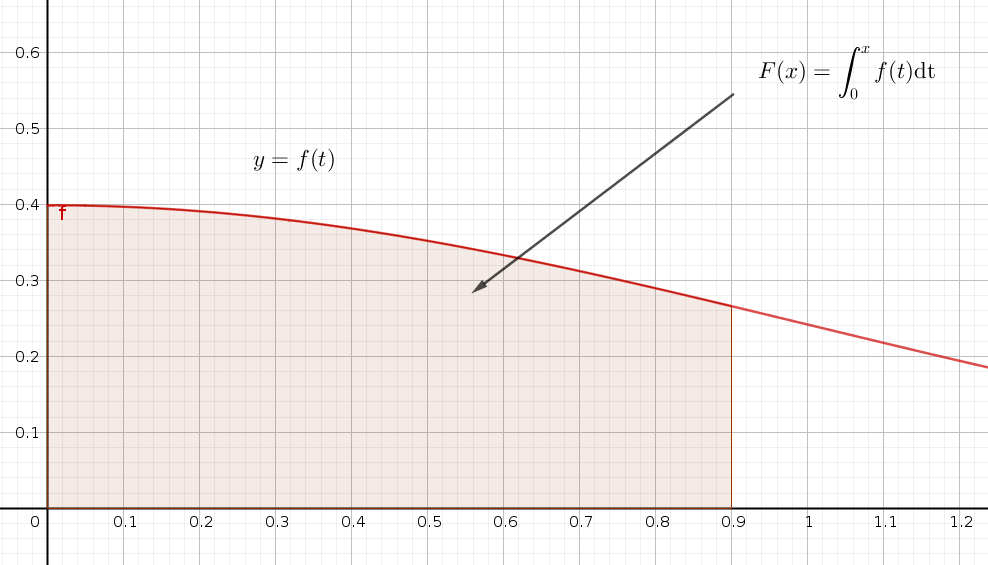
\includegraphics[scale=0.2]{images/exemple4.png}
\end{center}


\end{frame}


\begin{frame}
\frametitle{Exemple 5 Question 1}
\label{exemple5}

Soient les fonctions $f$ et $F$ continues sur $\Interoo{-\frac{\pi}{2}}{\frac{\pi}{2}}$ définies  par :
$$F(x)=\tan x - x \quad \text{et} \quad  f(x)=\tan^{2} x$$

$F$ est dérivable sur $\Interoo{-\frac{\pi}{2}}{\frac{\pi}{2}}$ et pour tout réel $x \in \Interoo{-\frac{\pi}{2}}{\frac{\pi}{2}}$, on a :

$$F'(x)= \frac{\cos( x )\times \cos(x) - \sin(x) \times (-\sin(x))}{\cos^{2}(x)} - 1 = \frac{\cos^{2}(x) + \sin^{2}(x)}{\cos^{2}(x)}-1$$

$$F'x()=  \frac{\sin^{2}(x)}{\cos^{2}(x)}= \tan^{2} x$$

$F$ est donc une primitive de $f$.





\end{frame}





\begin{frame}
\frametitle{Exemple 5 Question 2 a)}

Soient $g$ et $G$ les fonctions définies sur $\Interoo{0}{+\infty}$ par :
$$g(x)=\frac{1+\ln x}{x} \quad \text{et} \quad G(x)=\frac{1}{2}\left(\ln x \right)^{2}+\ln x $$

$G$ est dérivable sur $\Interoo{0}{+\infty}$, et pour tout réel $x>0$, on a :

$$G'(x)=\frac{1}{2} \times \frac{1}{x} \times 2 \ln(x) + \frac{1}{x}=\frac{1+\ln x}{x}$$
$$G'(x)=g(x)$$

$G$ et donc une primitive de $g$.

Notons que $M$ définie par $M(x)=G(x)+1$, a même dérivée $g$ que $G$ donc c'est une aussi une primitive de $g$. On peut remplacer $1$ par une constante $k$, toute fonction de la forme $G(x)+k$ est une primitive de $g$.

\end{frame}

\begin{frame}
\frametitle{Exemple 5 Question 2 b)}


$G(\text{e})=\frac{1}{2}\left(\ln \text{e} \right)^{2}+\ln \text{e} = \frac{3}{2}$.

La fonction $H$ définie par $H(x)=G(x) - G(\text{e}) = G(x) - \frac{3}{2}$, s'annule en $\text{e}$ et a pour dérivée $H'=G'=g$ donc c'est une primitive de $g$ qui s'annule en $\text{e}$.

Supposons  qu'il existe une autre primitive $N$ de $g$ qui s'annule en $\text{e}$, on a $(H-N)'=H'-N'=g-g=0$ donc $H-N$ est constante. De plus , $(H-N)(\text{e})=0$ donc $H-N=0$ donc $H=N$.

$H$ est donc l'unique primitive de $g$ qui s'annule en $\text{e}$.

\end{frame}


\begin{frame}
\frametitle{Exemple 6 Question 1) Partie 1}
\label{exemple6}
\renewcommand{\theenumi}{\alph{enumi}}
Chaque fonction $f$ considérée est continue donc admet des primitives sur son intervalle de définition.

\begin{enumerate}
 \item $f(x)= 4$ admet pour primitives les fonctions de la forme :
 $$F(x)=4x+k \text{ avec } k \text{ constante réelle}$$
 
  \item $f(x)= 0$ admet pour primitives les fonctions de la forme :
 $$F(x)=k \text{ avec } k \text{ constante réelle}$$
	
  \item  $f(x)= \frac{1}{\sqrt{x}}$ admet pour primitives les fonctions de la forme :
 $$F(x)= 2 \sqrt{x} + k \text{ avec } k \text{ constante réelle}$$
 
   \item  $f(x)= 3+x+x^4$ admet pour primitives les fonctions de la forme :
 $$F(x)=3x+\frac{1}{2}x^{2} + \frac{1}{5}x^{5} + k \text{ avec } k \text{ constante réelle}$$
 
 	
			  

\end{enumerate}

\end{frame}



\begin{frame}
\frametitle{Exemple 6 Question 1) Partie 2}
\renewcommand{\theenumi}{\alph{enumi}}

Chaque fonction $f$ considérée est continue donc admet des primitives sur son intervalle de définition.

\begin{enumerate}

 \item  $f(x)= \sin(2x)$ admet pour primitives les fonctions de la forme :
 $$F(x)=-\frac{1}{2}\cos(2x) +  k \text{ avec } k \text{ constante réelle}$$
 
\item  $f(x)=\cos(3x)$  admet pour primitives les fonctions de la forme :
 $$F(x)=\frac{1}{3}\sin(3x) +  k \text{ avec } k \text{ constante réelle}$$
 
 \item  $f(x)=\frac{1}{x^4}$ admet pour primitives les fonctions de la forme :
 $$F(x)=\frac{1}{-4+1}x^{-4+1} +  k \text{ avec } k \text{ constante réelle}$$

 

\end{enumerate}

\end{frame}



\begin{frame}
\frametitle{Exemple 6 Question 1) Partie 3}
\renewcommand{\theenumi}{\alph{enumi}}

Chaque fonction $f$ considérée est continue donc admet des primitives sur son intervalle de définition.

\begin{enumerate}

 \item  $f(x)=\e^{-2x}$ admet pour primitives les fonctions de la forme :
 $$F(x)=\frac{1}{-2}\e^{-2x} +  k \text{ avec } k \text{ constante réelle}$$
 
 \item  $f(x)= \frac{-1}{x}$ admet pour primitives les fonctions de la forme :
 $$F(x)=-\ln(\valabs{x}) +  k  = -\ln(-x) +  k \text{ avec } -x>0  \text{ et } k \text{ constante réelle}$$
 

\end{enumerate}

\end{frame}

\begin{frame}
\frametitle{Exemple 6 Question 2)}


Soit la fonction définie sur $\Interoo{0}{+\infty}$ par $F: x \mapsto x \ln x - x +1 $


Pour tout réel $x>0$, on a,en appliquant la formule de dérivation d'un produit pour $x \ln(x)$ : 

\begin{equation*}
F'(x)=x \times \frac{1}{x} + 1 \times \ln(x) -1=\ln(x)
\end{equation*}

$F$ est donc une primitive de la fonction $\ln$. La primitive $G$ de $\ln$ qui s'annule en $\sqrt{\text{e}}$. est donc de la forme $G(x)=F(x)+k$. Il suffit de déterminer $k$ en évaluant $G$ en $\sqrt{\text{e}}$: 
$$G(\sqrt{\text{e}})=F(\sqrt{\text{e}})+k= \frac{1}{2}\sqrt{\text{e}}-\sqrt{\text{e}}+1+k=0 \Leftrightarrow k = \frac{1}{2}\sqrt{\text{e}}-1$$
La primitive de $\ln$ qui s'annule en $\sqrt{\text{e}}$ est donc $G(x)=x \ln x - x +\frac{1}{2}\sqrt{\text{e}}$.
\end{frame}

\begin{frame}
\frametitle{Exemple 6 Question 2)}

Soit la fonction définie sur $\Interoo{0}{+\infty}$ par $F: x \mapsto x \ln x - x +1 $


Pour tout réel $x>0$, on a,en appliquant la formule de dérivation d'un produit pour $x \ln(x)$ : 

\begin{equation*}
F'(x)=x \times \frac{1}{x} + 1 \times \ln(x) -1=\ln(x)
\end{equation*}

$F$ est donc une primitive de la fonction $\ln$. La primitive $G$ de $\ln$ qui s'annule en $\sqrt{\text{e}}$. est donc de la forme $G(x)=F(x)+k$. Il suffit de déterminer $k$ en évaluant $G$ en $\sqrt{\text{e}}$: 
$$G(\sqrt{\text{e}})=F(\sqrt{\text{e}})+k= \frac{1}{2}\sqrt{\text{e}}-\sqrt{\text{e}}+1+k=0 \Leftrightarrow k = \frac{1}{2}\sqrt{\text{e}}-1$$
La primitive de $\ln$ qui s'annule en $\sqrt{\text{e}}$ est donc $G(x)=x \ln x - x +\frac{1}{2}\sqrt{\text{e}}$.
\end{frame}



\begin{frame}
\frametitle{Exemple 7 Partie 1}

\label{exemple7}

\begin{enumerate}

 \item  $f(x)=x^2-2x-1-\frac{1}{x^2}-\frac{1}{x}+\text{e}^{x}$admet pour primitives les fonctions de la forme :
 $$F(x)=\frac{x^{3}}{3}-x^{2}-x+\frac{1}{x}-\ln(\valabs{x})+\text{e}^{x}+  k \text{ avec } k \text{ constante réelle}$$
 
\item  $f(x)=\cos(4x-1)-2\sin(2x)$   admet pour primitives les fonctions de la forme :
 $$F(x)=\frac{1}{4}\sin(4x-1) + 2\times \frac{1}{2} \cos(2x) +  k \text{ avec } k \text{ constante réelle}$$
 
 \item   $f(x)=\frac{\e^{731x}}{(\e^{731x}+1)^2}$  est de la forme $\frac{1}{731}\frac{u'}{u^{2}}$ avec $u(x)=\e^{731x}+1$, donc admet pour primitives les fonctions de la forme :
 $$F(x)=-\frac{1}{u(x)}+k=-\frac{1}{731}\frac{1}{\e^{731x}+1} +  k = \text{ avec } k \text{ constante réelle}$$


			
\end{enumerate}

\end{frame}




\begin{frame}
\frametitle{Exemple 7 Partie 2}

\begin{enumerate}



 \item   $f(x)=\frac{\e^{-x}}{\e^{-x}+1}$   est de la forme $-\frac{u'}{u}$ avec $u(x)=\e^{-x}+1$, donc admet pour primitives les fonctions de la forme :
 $$F(x)=-\ln(\valabs{u(x)})+k=-\ln(\valabs{\e^{-x}+1} )  +  k  = -\ln(\e^{-x}+1 )  +  k  \text{ , } k \in \R$$


 \item   $f(x)=\frac{x}{\text{e}^{x^2}}=x \text{e}^{-x^2}$    est de la forme $-\frac{1}{2}u'\text{e}^{u}$ avec $u(x)=-x^2$, donc admet pour primitives les fonctions de la forme :
 $$F(x)=-\frac{1}{2} \text{e}^{u(x)} +k=-\frac{1}{2} \text{e}^{-x^2}  +  k    \text{ , } k \in \R$$




 

			
\end{enumerate}

\end{frame}



\begin{frame}
\frametitle{Exemple 7 Partie 3}

\begin{enumerate}

 \item   $f(x)=\frac{1}{x \ln x}=\frac{\frac{1}{x}}{\ln(x)}$    est de la forme $\frac{u'}{u}$ avec $u(x)=\ln(x)$, donc admet pour primitives les fonctions de la forme :
 $$F(x)=\ln(\valabs{u(x)}) +k=\ln(\valabs{\ln(x)})  +  k    \text{ , } k \in \R$$
 
 Sur $\Interoo{0}{1}$, on a $\ln(x)<0$ donc $F(x)=\ln(-\ln(x))  +  k$.
 
  Sur $\Interoo{1}{+\infty}$, on a $\ln(x)>0$ donc $F(x)=\ln(\ln(x))  +  k$.

 \item   $f(x)=\cos(x)\text{e}^{\sin(x)}$    est de la forme $u'\text{e}^{u}$ avec $u(x)=\sin(x)$, donc admet pour primitives les fonctions de la forme :
 $$F(x)=\text{e}^{u(x)} +k=\text{e}^{\sin(x)} +k    \text{ , } k \in \R$$
 
 
 \item   $f(x)=\frac{1}{x}\times \left(\ln x\right)^2$    est de la forme $u'u^{2}$ avec $u(x)=\ln(x)$, donc admet pour primitives les fonctions de la forme :
 $$F(x)=\frac{1}{3}u^{3}(x)+k=\frac{1}{3}(\ln(x))^{3} +k    \text{ , } k \in \R$$
 

			
\end{enumerate}

\end{frame}



\begin{frame}
\frametitle{Exemple 8 Partie 1}
\label{exemple8}
On considère les  courbes d'équations $y=1$, $y=x$ et $y=x^2$ sur l'intervalle $\Interff{0}{1}$.

Pour tout réel $x \in \Interff{0}{1}$, on a :
\begin{align*}
0 & \leqslant x \leqslant  1 \\
\intertext{on multiplie par $x \geqslant 0$}
0 & \leqslant x^{2}   \leqslant x  \leqslant 1
\end{align*}




\end{frame}


\begin{frame}
\frametitle{Exemple 8 Figure }


\begin{center}
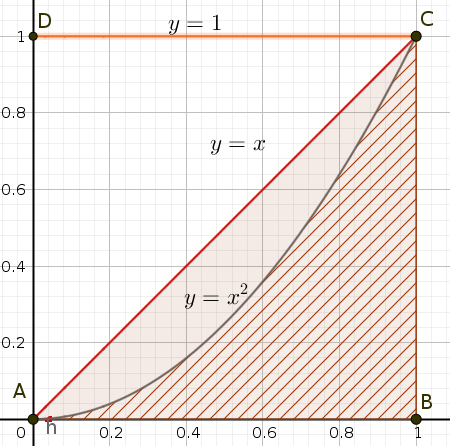
\includegraphics[scale=0.3]{images/exemple8.png}
\end{center}

\end{frame}


\begin{frame}
\frametitle{Exemple 8 Partie 2 }

Puisque pour tout réel $x \in \Interff{0}{1}$, on a $0  \leqslant x^{2}   \leqslant x  \leqslant 1$, on en déduit que : la courbe d'équation $y=x^2$ est donc en dessous de la droite d'équation $y=x$, elle même en-dessous de la droite d'équation $y=1$.

Par définition de l'intégrale d'une fonction continue positive comme aire du domaine  \og{} sous sa courbe \fg{} (délimité par sa courbe, l'axe des abscisses et les deux droites parallèles à l'axe des ordonnées passant par les bornes de l'intervalle), on en déduit que :

$$I= \int_{0}^{1}x^2 \ \dx \leqslant K= \int_{0}^{1} x \ \dx  \leqslant J = \int_{0}^{1} 1 \ \dx$$
 

\end{frame}



\begin{frame}
\frametitle{Exemple 8 Partie 3 }


De plus, par additivité des aires, l'intégrale   $L=\int_{0}^{1} 1-x^2  \ \dx$ représente l'aire du domaine entre la droite d'équation $y=1$ et la courbe d'équation $y=x^2$, de même   $M=\int_{0}^{1} x-x^2  \ \dx$ représente l'aire du domaine entre la droite d'équation $y=x$ et la courbe d'équation $y=x^2$.

On peut noter que pour tout réel $x \in \Interff{0}{1}$, on a $0  \leqslant x^{2}   \leqslant x  \leqslant 1$, donc $0 \leqslant x - x^{2} \leqslant 1- x^{2}$ et donc $M \leqslant L$.  

\end{frame}




\begin{frame}
\frametitle{Exemple  9 Partie 1}
\label{exemple9}

Calculer les intégrales suivantes :

			\begin{enumerate}
			\item $\int_{-1}^{1}\frac{\text{e}^x}{\sqrt{\text{e}^x+1}} \ \dx = \left[2\sqrt{\text{e}^x+1}\right]_{-1}^{1}=2\sqrt{\text{e}^{1}+1}-2\sqrt{\text{e}^{-1}+1}$  ;
				\item $\int_{2}^{4}\frac{1}{(2x-1)^4} \ \dx =   \left[\frac{1}{2}\times \frac{1}{-4+1}(2x-1)^{-4+1}\right]_{2}^{4}$
				
				$\int_{2}^{4}\frac{1}{(2x-1)^4} \ \dx = \frac{1}{2}\times \frac{1}{-4+1}(7)^{-4+1}- \frac{1}{2}\times \frac{1}{-4+1}(3)^{-4+1}$
				
				\item $\int_{0}^{2\pi} \cos\left( \theta \right)  \ d\theta  =  \left[\sin\left( \theta \right)\right]_{0}^{2\pi}=0-0=0$;
				
				\item $\int_{0}^{\pi} \cos \left( 2\theta \right)  \ d\theta =  \left[\frac{1}{2}\sin\left( 2\theta \right)\right]_{0}^{\pi}=0-0=0$;
							
				\item $\int_{-4}^{-2}(3x-1)^6 \dx = \left[\frac{1}{3}\times \frac{1}{7}(3x-1)^{7}\right]_{-4}^{-2}=\frac{1}{21}\left(-7^{7}+13^{7} \right)$ ;
				\item $\int_{0}^{x}\sin^2(t) \ \dt$. Il faut linéariser $\sin^{2}(t)$ avec les formules de duplication du sinus (voir chapitre sur les complexes Partie 2) : $\sin^{2}(t)=\frac{1-\cos(2t)}{2}$ donc :
				
				$\int_{0}^{x}\sin^2(t) \ \dt = \int_{0}^{x}\frac{1-\cos(2t)}{2}\ \dt  = \left[\frac{t-0,5\sin(2t)}{2}\right]_{0}^{x}= \frac{x-0,5\sin(2x)}{2}-0$
				
		
			\end{enumerate}

\end{frame}




\begin{frame}
\frametitle{Exemple  9 Partie 2}


Calculer les intégrales suivantes :

			\begin{enumerate}
						
				\item $\int_{e}^{e^3} \frac{1}{x \ln x} \ \dx = \left[\ln(\valabs{\ln(x)})\right]_{e}^{e^3}=\ln(\ln(3))- \ln(1)=\ln(\ln(3))$
				\item $\int_{0}^{x} \frac{1}{1+\text{e}^t}  \ \dt$ Ici il faut transformer l'expression pour faire apparaître une forme $\frac{u'}{u}$ (ici $-\frac{u'}{u}$). L'astuce classique avec l'exponentielle : $\text{e}^{t}\times \text{e}^{-t}=1$.

$\int_{0}^{x} \frac{1}{1+\text{e}^t}  \ \dt = \int_{0}^{x} \frac{\text{e}^{-t} \times 1}{\text{e}^{-t}(1+\text{e}^t)}  \ \dt =\int_{0}^{x} \frac{\text{e}^{-t} \times 1}{\text{e}^{-t}+1}  \ \dt$

Puis : 	$\int_{0}^{x} \frac{\text{e}^{-t}  }{\text{e}^{-t}+1}  \ \dt=\left[-\ln(\valabs{\text{e}^{-t}+1})\right]_{0}^{x}=-\ln(\text{e}^{-x}+1) + \ln(2)$

				
				\item $\int_{2}^{e} \frac{1}{x(\ln(x))^2}  \ \dx = \left[-\frac{1}{\ln(x)}\right]_{2}^{e}=-\frac{1}{\ln(e)}+\frac{1}{\ln(2)} =\frac{1}{\ln(2)}-1$ Ici on a écrit $\frac{1}{x(\ln(x))^2}=\frac{u'(x)}{u^{2}(x)}$ avec $u(x)=\ln(x)$ pour déterminer une primitive qui est $-\frac{1}{u(x)}$.
			\end{enumerate}

\end{frame}

\begin{frame}
\frametitle{Exemple  10 Partie  1}
\label{exemple10}


Le demi-cercle $\Gamma$ de rayon $1$, représenté sur la figure ci-dessous, a pour équation $y=\sqrt{1-x^2}$.

La partie grisée est comprise entre l'axe des abscisses d'équation $y=0$ et la courbe $\courbe{f}$ de la fonction $f$ définie sur  $\Interff{-1}{1}$ par 	$f(x)=\frac{1}{2}(1-x)\sqrt{1-x^2}$.

\begin{center}
\begin{tikzpicture}[xmin=-1.5,xmax=1.5,ymin=-0.5,ymax=1.5,scale=1.5]
\fenetre
\draw[thick] plot[samples=1000,smooth,domain=-1:0.99] (\x,{sqrt(1 - \x * \x)});
\draw[thick] plot[samples=100,smooth,domain=0.99:1] (\x,{sqrt(1 - \x * \x)});
\filldraw[thick, fill=gray!50] plot[thick,samples=1000,smooth,domain=-1:1] (\x,{sqrt(1 - \x * \x)*(1-\x)/2}) -- (-1,0);
\axes
\draw[thick] (0,1) node[above left] {$1$};
\draw[thick] (1,0) node[below right] {$1$};
\draw[thick] (-1,0) node[below left] {$-1$};
\draw (0,0) node [below left] {O};
\draw (0.71, 0.71) node[above] {$\Gamma$};
\draw (0.2, 0.4) node[above right] {$\courbe{f}$};
\end{tikzpicture}
\end{center}

\end{frame}



\begin{frame}
\frametitle{Exemple  10 Partie 2}

\begin{itemize}
	\item  $\displaystyle\int_{-1}^{1}\sqrt{1-x^2}\dx$  est l'aire du demi-disque de rayon $1$ donc c'est $\frac{1}{2}\times \pi \times 1^{2}=\frac{\pi}{2}$.
	\item Pour tout réel $x \in \Interff{-1}{1}$, si on note $g(x)= x\sqrt{1-x^2}$, on a$g(-x)=-g(x)$ donc par symétrie centrale de centre l'origine du repère  $\int_{-1}^{0}g(x)\dx$ est l'opposé de l'aire du domaine sous la courbe de $g$  sur l'intervalle $\Interff{0}{1}$.

On a donc $\int_{-1}^{0}g(x)\dx = -\int_{0}^{1}g(x)\dx \Leftrightarrow  \displaystyle\int_{-1}^{0}x\sqrt{1-x^2}\dx=-\displaystyle\int_{0}^{1}x\sqrt{1-x^2}\dx $.


\end{itemize}


\end{frame}



\begin{frame}
\frametitle{Exemple  10 Partie 3}
%
%
\begin{itemize}
	
\item $\displaystyle\int_{-1}^{1}f(x)\dx = \displaystyle\int_{-1}^{1}\frac{1}{2}(1-x)\sqrt{1-x^2} \dx =\frac{1}{2}\displaystyle\int_{-1}^{1}(1-x)\sqrt{1-x^2} \dx$ par linéarité.

De nouveau par linéarité, on a $\displaystyle\int_{-1}^{1}f(x)\dx =\frac{1}{2}\left(\int_{-1}^{1}\sqrt{1-x^2} \dx - \int_{-1}^{1}x\sqrt{1-x^2} \dx\right) = \frac{1}{2}\left(\frac{\pi}{2}-  \int_{-1}^{1}x\sqrt{1-x^2}\dx \right) $.

En appliquant la relation de Chasles, on a  $ \int_{-1}^{1}x\sqrt{1-x^2}\dx = \int_{-1}^{0}x\sqrt{1-x^2}\dx + \int_{0}^{1}x\sqrt{1-x^2}\dx$

D'après la propriété d'antisymétrie de la question 2), il vient $-\int_{0}^{1}x\sqrt{1-x^2}\dx +  \int_{0}^{1}x\sqrt{1-x^2}\dx=0$.

Finalement, on a  $\boxed{\displaystyle\int_{-1}^{1}f(x)\dx = \frac{\pi}{4}}$.

\end{itemize}


\end{frame}



\begin{frame}
\frametitle{Exemple  11}
\label{exemple11}

Soient $f$ et $g$ deux fonctions continues sur $\Interff{1}{5}$, on donne :
$$I=\int_{1}^{2} f(x)\dx=-3   \qquad J=\int_{5}^{2} f(x)\dx=2 \qquad  K=\int_{1}^{5} g(x)\dx=12$$
Calculer $L=\int_{1}^{5} f(x)\dx$, $M=\int_{1}^{5} (f(x)+g(x))\dx$ puis $N=\int_{1}^{5} (2f(x)-3g(x))\dx$.

\begin{itemize}
	
\item  On applique la relation de Chasles : 

$L=\int_{1}^{5} f(x)\dx =\int_{1}^{2} f(x)\dx + \int_{2}^{5} f(x)\dx  = \int_{1}^{2} f(x)\dx  - \int_{5}^{2} f(x)\dx = I - J=-5 $

\item On applique la propriété de linéarité  :

$M=\int_{1}^{5} (f(x)+g(x))\dx = \int_{1}^{5} f(x)\dx  + \int_{1}^{5} g(x)\dx  = L + K = -5+12=7$


\item On applique la propriété de linéarité  :

$N=\int_{1}^{5} (2f(x)-3g(x))\dx=2\int_{1}^{5}f(x)\dx - 3 \int_{1}^{5}g(x)\dx = 2 \times (-5) -3 \times (12)= -46$

\end{itemize}


\end{frame}


\begin{frame}
\frametitle{Exemple  12 Question 1)}
\label{exemple12}


Déterminer le signe des intégrales suivantes :

\begin{itemize}
\item $I=\integralex{\frac{1}{2}}{1}{\ln x}$

Pour tout réel $x \in \Interff{\frac{1}{2}}{1}$, on a  :
\pause\begin{align*}
  0   & \geqslant \ln(x) \\
 \intertext{donc par croissance de l'intégrale on a : }
 0 & \geqslant \integralex{\frac{1}{2}}{1}{\ln x}
\end{align*}

\item $\integralex{1}{0}{x^{2}}$
\item $\integralex{1}{\frac{1}{\text{e}}}{\ln x}$
\end{itemize}



\end{frame}



\begin{frame}
\frametitle{Exemple  12 Question 1)}



Déterminer le signe des intégrales suivantes :

\begin{itemize}
 \item $I=\integralex{1}{0}{x^{2}}$

Pour tout réel $x \in \Interff{0}{1}$, on a  :
\pause\begin{align*}
  0   & \leqslant x^{2} \\
 \intertext{donc par croissance de l'intégrale on a : }
 0 & \leqslant \integralex{0}{1}{x^{2}} \\ 
  \intertext{donc par linéarité : }
   0 & \geqslant -\integralex{0}{1}{x^{2}} \\ 
      0 & \geqslant \integralex{1}{0}{x^{2}} \\ 
\end{align*}


\end{itemize}



\end{frame}



\begin{frame}
\frametitle{Exemple  12 Question 1)}



Déterminer le signe des intégrales suivantes :

\begin{itemize}
\item $I=\integralex{1}{\frac{1}{\text{e}}}{\ln x}$

Pour tout réel $x \in \Interff{\frac{1}{\text{e}}}{1}$, on a  :
\pause \begin{align*}
  0   & \geqslant \ln x  \\
 \intertext{donc par croissance de l'intégrale on a : }
 0 & \geqslant \integralex{\frac{1}{\text{e}}}{1}{\ln x} \\ 
  \intertext{donc par linéarité : }
   0 & \leqslant -\integralex{\frac{1}{\text{e}}}{1}{\ln x}\\ 
      0 & \leqslant \integralex{1}{\frac{1}{\text{e}}}{\ln x} \\ 
\end{align*}


\end{itemize}



\end{frame}




\begin{frame}
\frametitle{Exemple  12 Question 2)}



Soit $\suite{u}$ la suite définie pour tout entier $n \geqslant 1$ par $u_n=\integralex{0}{1}{\ln\left(1+x^n\right)}$

Pour étudier le sens de variation de la suite $\suite{u}$, deux méthodes sont possibles :




\end{frame}


\begin{frame}
\frametitle{Exemple  12 Question 2)}
\fbox{\textbf{Méthode 1 :On étudie le signe de $u_{n+1}-u_{n}$} }



Pour tout entier $n \geqslant 1$, on a :
\pause \begin{align*}
u_{n+1}-u_{n} &= \integralex{0}{1}{\ln\left(1+x^{n+1}\right)} - \integralex{0}{1}{\ln\left(1+x^{n}\right)} \\
\intertext{donc par linéarité :}
u_{n+1}-u_{n} &= \integralex{0}{1}{\ln\left(1+x^{n+1}\right)-\ln\left(1+x^{n}\right)}
\intertext{Or pour tout entier $n \geqslant 1$ et tout réel $x \in \Interff{0}{1}$, on a $0 \leqslant x \leqslant 1$ donc en multipliant tous les membres par $x^{n} \geqslant 0$,   $0 \leqslant x^{n+1} \leqslant x^{n}$  puis par croissance de $\ln$,  $\ln(1) \leqslant \ln(1+x^{n+1}) \leqslant \ln(1+x^{n})$ donc $ \ln(1+x^{n+1}) - \ln(1+x^{n})\leqslant 0$ et par croissance de   l'intégrale :
}
u_{n+1}-u_{n} &= \integralex{0}{1}{\ln\left(1+x^{n+1}\right)-\ln\left(1+x^{n}\right)} \leqslant 0
\end{align*}
On en déduit que la suite $\suite{u}$ est décroissante.




\end{frame}



\begin{frame}
\frametitle{Exemple  12 Question 2)}
\fbox{\textbf{Méthode 2 : $u_{n+1}\leqslant u_{n}$ par croissance de l'intégrale} }

Le principe est de comparer les expressions sous le signe d'intégration et d'en déduire les inégalités sur les intégrales par croissance de l'intégrale. C'est similaire à la méthode précédente mais avec une rédaction plus légère. Pour tout entier $n \geqslant 1$, pour tout réel $x \in \Interff{0}{1}$,  on a :
\pause \begin{align*}
x & \leqslant 1 \\
\intertext{on multiplie les deux membres par $x^{n}  \geqslant 0$ puis   on ajoute $1$ et on compose par le $\ln$ qui est croissant, on en déduit que :
}
\ln\left(1+x^{n+1}\right) &\leqslant \ln\left(1+x^{n}\right)
\end{align*}

Par croissance de l'intégrale, il vient :
$$\integralex{0}{1}{\ln\left(1+x^{n+1}\right)} \leqslant \integralex{0}{1}{\ln\left(1+x^{n}\right)}$$
et donc $u_{n+1}  \leqslant u_{n}$  et  la suite $\suite{u}$ est décroissante.




\end{frame}





\begin{frame}
\frametitle{Exemple  12 Question 2)}
Démontrer que pour tout entier $n \geqslant 1$, on a $0 \leqslant u_{n} \leqslant \ln 2$ (début).

On utilise la croissance de l'intégrale. Pour tout entier $n \geqslant 1$, pour tout réel $x \in \Interff{0}{1}$,  on a $0 \leqslant 1+x^{n}  \leqslant 2$ donc par croissance de la fonction $\ln$ :

\pause \begin{align*}
0 & \leqslant \ln\left(1+x^{n}\right) \leqslant \ln(2) \\
\intertext{par croissance de l'intégrale : }
 \integralex{0}{1}{0} & \leqslant \integralex{0}{1}{\ln\left(1+x^{n}\right)}  \leqslant \integralex{0}{1}{\ln(2)} \\
\intertext{par linéarité : }
 0 \times \integralex{0}{1}{1} & \leqslant \integralex{0}{1}{\ln\left(1+x^{n}\right)}  \leqslant \ln(2) \times \integralex{0}{1}{1} \\
\end{align*}





\end{frame}





\begin{frame}
\frametitle{Exemple  12 Question 2)}
Démontrer que pour tout entier $n \geqslant 1$, on a $0 \leqslant u_{n} \leqslant \ln 2$ (fin):

\pause \begin{align*}
\intertext{par linéarité : }
 0 \times \integralex{0}{1}{1} & \leqslant \integralex{0}{1}{\ln\left(1+x^{n}\right)}  \leqslant \ln(2) \times \integralex{0}{1}{1} \\
0 & \leqslant \integralex{0}{1}{\ln\left(1+x^{n}\right)}  \leqslant \ln(2)  \\
0 & \leqslant u_{n}  \leqslant \ln(2)
\end{align*}

La suite $\suite{u}$ est donc minorée par $0$, comme elle est décroissante (question précédente), elle converge d'après le théorème de convergence monotone.




\end{frame}





\begin{frame}
\frametitle{Exemple  12 Question 3)}
Démontrer que pour tout entier $n \geqslant 1$, pour tout réel $x \in \Interff{0}{1}$ on a : $0 \leqslant \ln\left(1+x^n\right) \leqslant  x^n  $ . En déduire la limite de la  suite $\suite{u}$.

On utilise encore la croissance de l'intégrale.

Pour tout entier $n \geqslant 1$, pour tout réel $x \in \Interff{0}{1}$ :

on a $\ln(1+x) \leqslant x$  d'après une propriété de la fonction $\ln$ (courbe de $\ln$ en-dessous de toutes ses tangentes et la droite d'équation $y=x+1$ est sa tangente au point d'abscisse $0$). On peut remplacer $x$ par $x^{n}$  : $0 \leqslant \ln(1+x^{n}) \leqslant x^{n}$. Par croissance de l'intégrale, on a :

\pause \begin{align*}
0 \leqslant \integralex{0}{1}{\ln(1+x^{n}) } & \leqslant \integralex{0}{1}{x^{n}} \\
0 \leqslant \integralex{0}{1}{\ln(1+x^{n}) } & \leqslant \left[\frac{x^{n+1}}{n+1} \right]_{0}^{1} \\
0 \leqslant \integralex{0}{1}{\ln(1+x^{n}) } & \leqslant \frac{1}{n+1}\\
\end{align*}

On a $\limitesuite{\frac{1}{n+1}}=0$ donc d'après le théorème des gendarmes, on a $\limitesuite{u_{n}}=0$.




\end{frame}



\begin{frame}
\frametitle{Exemple  12 Question 3)}
\pause \begin{align*}
0 \leqslant \integralex{0}{1}{\ln(1+x^{n}) } & \leqslant \integralex{0}{1}{x^{n}} \\
0 \leqslant \integralex{0}{1}{\ln(1+x^{n}) } & \leqslant \left[\frac{x^{n+1}}{n+1} \right]_{0}^{1} \\
0 \leqslant \integralex{0}{1}{\ln(1+x^{n}) } & \leqslant \frac{1}{n+1}\\
0 \leqslant u_{n} & \leqslant \frac{1}{n+1}\\
\end{align*}

On a $\limitesuite{\frac{1}{n+1}}=0$ donc d'après le théorème des gendarmes, on a $\limitesuite{u_{n}}=0$.




\end{frame}





\begin{frame}
\frametitle{Exemple  13 Partie 1}

Soit $f$ définie sur $\Interfo{0}{+\infty}$ par $f(t)=\frac{1}{\sqrt{2\pi}}\text{e}^{-\frac{t^2}{2}}$.
\begin{itemize}
\item Démontrons que pour tout $t \in \Interfo{2}{+\infty}$ on a  
 $0 \leqslant f(t) \leqslant \frac{1}{\sqrt{2\pi}}\text{e}^{-t}$.


Pour tout  $t \in \Interfo{2}{+\infty}$ on a :
\pause \begin{align*}
2 &\leqslant t \\
2t & \leqslant t^{2} \\
-t & \geqslant -\frac{t^2}{2} \\
\intertext{par croissance de la fonction exponentielle : }
\text{e}^{-t}  &\geqslant \text{e}^{-\frac{t^2}{2}} \\
\frac{1}{\sqrt{2\pi}}\text{e}^{-t}  &\geqslant \frac{1}{\sqrt{2\pi}}\text{e}^{-\frac{t^2}{2}}
\end{align*}


\end{itemize}

\end{frame}




\begin{frame}
\frametitle{Exemple  13 Partie 2}

Soit $f$ définie sur $\Interfo{0}{+\infty}$ par $f(t)=\frac{1}{\sqrt{2\pi}}\text{e}^{-\frac{t^2}{2}}$.

\pause \begin{itemize}
\item  Pour tout entier $n \geqslant 2$ on a : 
\pause \begin{align*}
0 \leqslant  \frac{1}{\sqrt{2\pi}}\text{e}^{-\frac{t^2}{2}}   &\leqslant  \frac{1}{\sqrt{2\pi}}\text{e}^{-t} \\
\intertext{donc par croissance de l'intégrale :}
0 \leqslant \integralet{2}{n}{f(t)} & \leqslant \integralet{2}{n}{\frac{1}{\sqrt{2\pi}}\text{e}^{-t} } \\
0 \leqslant \integralet{2}{n}{f(t)} & \leqslant \left[-\frac{1}{\sqrt{2\pi}}\text{e}^{-t}  \right]_{2}^{n} \\ 
0 \leqslant \integralet{2}{n}{f(t)} & \leqslant \frac{1}{\sqrt{2\pi}}\text{e}^{-2}-  \frac{1}{\sqrt{2\pi}}\text{e}^{-n} \\
0 \leqslant \integralet{2}{n}{f(t)} & \leqslant \frac{1}{\sqrt{2\pi}}\text{e}^{-2}
\end{align*}
\end{itemize}
\end{frame}



\begin{frame}
\frametitle{Exemple  13 Partie 3}

Démontrons que la suite $\suite{u}=\Suite{\integralet{2}{n}{f(t)}}{n \geqslant 2}$ est croissante.

Pour tout entier $n \geqslant 2$ : 

\pause \begin{align*}
\integralet{2}{n+1}{f(t)}  - \integralet{2}{n}{f(t)}  &= \integralet{2}{n+1}{f(t)}  + \integralet{n}{2}{f(t)} \\
\integralet{2}{n+1}{f(t)}  - \integralet{2}{n}{f(t)}  &= \integralet{n}{2}{f(t)} +\integralet{2}{n+1}{f(t)}  \\
\integralet{2}{n+1}{f(t)} -\integralet{2}{n}{f(t)}  &= \integralet{n}{n+1}{f(t)}
\end{align*}
Pour tout entier $n \geqslant 2$, on a $0 \leqslant f(t)$ sur $\Interff{n}{n+1}$, donc par croissance de l'intégrale :
$
0 \leqslant \integralet{n}{n+1}{f(t)}
$

Pour tout entier $n \geqslant 2$, on a donc $u_{n+1}-u_{n} \geqslant 0$ et donc la suite $\suite{u}$ est croissante. Comme elle est majorée par $\frac{1}{\sqrt{2\pi}}\text{e}^{-2}$, elle converge d'après le théorème de convergence monotone.
\end{frame}
%




\begin{frame}
\frametitle{Exemple  14}
\label{exemple14}
On considère les fonctions $f$ et $g$ définies sur l'intervalle [0~;~16] par

\[f(x) = \ln(x + 1)\quad  \text{et}\quad g(x) = \ln(x + 1) + 1 - \cos(x).\]

Dans un repère du plan \Oij, on note $\mathcal{C}_f$ et $\mathcal{C}_g$ les courbes représentatives des fonctions $f$ et $g$. Ces courbes sont données  ci-dessous.


\begin{center}
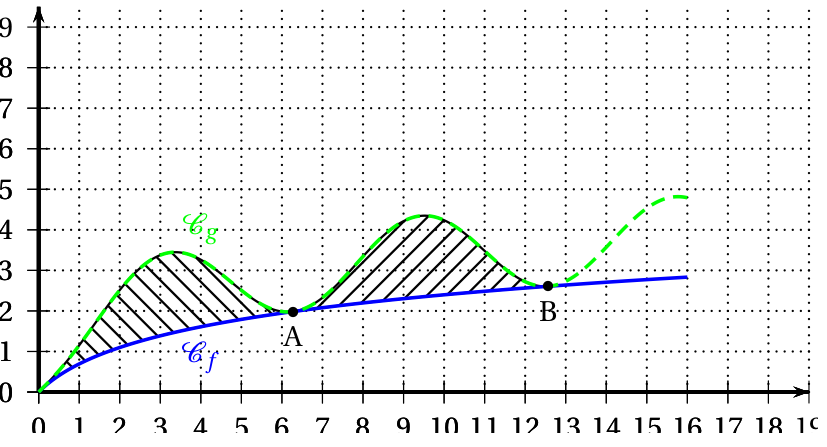
\includegraphics[scale=0.2]{images/exemple14.png}
\end{center}
\end{frame}



\begin{frame}
\frametitle{Exemple  14}

Pour tout  $x \in [0~;~16]$, on a $g(x)-f(x) =  1 - \cos(x)$.

 Or $1-\cos(x) \geqslant 0$, donc $g(x)-f(x)\geqslant 0$.

 De plus  $g(x)-f(x) = 0 \Leftrightarrow 1 = \cos(x) \Leftrightarrow x = k2\pi \text{ avec } k \in \Z$

Sur l'intervalle $[0~;~16]$, on a donc $g(x)-f(x) = 0 \Leftrightarrow \begin{cases} x = 0 \\ x = 2 \pi \\ x = 4 \pi \end{cases}$.

Le domaine hachuré sur le graphique est l'aire entre les courbes de $f$ et de $g$ sur $[0~;~16]$.

Sachant que $g \geqslant f$, cette aire est égale à l'intégrale :
\pause \begin{align*}
\integralex{0}{4\pi}{g(x)-f(x)} &=\integralex{0}{4\pi}{1-\cos(x)}\\
 \integralex{0}{4\pi}{g(x)-f(x)} &=\left[x-\sin(x)\right]_{0}^{4\pi} = 4\pi
\end{align*}

\end{frame}

 

\begin{frame}
\frametitle{Exemple  15 Partie 1}
Pour $t>0$ la vitesse d'un mobile est $v(t)=\frac{1}{t^2}+\frac{1}{t}$ ( en $\text{m}.\text{s}^{-1}$).
\begin{enumerate}
\item La distance parcourue entre les instants $t=1$ et $t=\text{e}^2$ (en s) est égale à :

\begin{align*}
\integralet{1}{\text{e}^2}{v(t)} &= \integralet{1}{\text{e}^2}{\frac{1}{t^2}+\frac{1}{t}} \\
\integralet{1}{\text{e}^2}{v(t)} &= \left[-\frac{1}{t}+\ln(t)\right]_{1}^{\text{e}^2} \\
\integralet{1}{\text{e}^2}{v(t)} &= 2 -\text{e}^{-2}+1 \text{mètres}
\end{align*}


\item  La vitesse moyenne du mobile entre les instants $t=1$ et $t=\text{e}^2$ est est égale à :
$
\integralet{1}{\text{e}^2}{v(t)} = \frac{1}{\text{e}^2-1}\integralet{1}{\text{e}^2}{\frac{1}{t^2}+\frac{1}{t}}= \frac{3 -\text{e}^{-2}}{\text{e}^2-1} \text{mètres par seconde}$

\end{enumerate}
\end{frame}




\begin{frame}
\frametitle{Exemple  16}
\label{exemple16}

\begin{enumerate}
\item Valeur moyenne de la fonction  $g$ définie sur $\Interff{-1}{1}$ par \mbox{$g(x)=\text{e}^{-x}$}. 
\begin{equation*}
\frac{1}{2}\integralex{-1}{1}{g(x)} = \frac{1}{2} \left[-\text{e}^{-x}\right]_{1}^{2}= \frac{1}{2}\left(\text{e}^{-1}- \text{e}^{-2}  \right)
\end{equation*}
\item  Soit $f$ une fonction continue sur un intervalle $\Interff{a}{b}$.
On suppose que pour tout $x \in \Interff{a}{b}$ on a : $m \leqslant f(x) \leqslant M$ . Par croissance de l'intégrale :
\begin{align*}
m \integralex{a}{b}{1}  \leqslant \integralex{a}{b}{f(x)}  & \leqslant M \integralex{a}{b}{1}  \\
m (b-a) \leqslant \integralex{a}{b}{f(x)}  & \leqslant M(b-a) \\
 m \leqslant \frac{1}{b-a}\integralex{a}{b}{f(x)}  &\leqslant M
\end{align*}
\end{enumerate}
\end{frame}



\begin{frame}
\frametitle{Exemple  16 Partie 2 }
\label{exemple16}
Soit $f$ la fonction définie sur l'intervalle  $\text{I}=\Interff{-1}{1}$ par $f(x)=(x+1)\text{e}^{-x}+1$
\begin{enumerate}
\item  Pour tout réel $x$, on a $f'(x)=\text{e}^{-x} - \text{e}^{-x}(x+1)=-x\text{e}^{-x}$.

$f'(x)$ est donc du signe de $-x$ sur $\Interff{-1}{1}$  donc positive sur $\Interff{-1}{0}$ puis négative sur $\Interff{0}{1}$, donc $f$ est croissante sur  $\Interff{-1}{0}$ puis décroissante sur $\Interff{0}{1}$.

De plus, $f(-1)=1$ et $f(1)=2\text{e}^{-1}+1$, donc le minimum de $f$ sur $\Interff{0}{1}$ est $f(-1)$ et le maximum est $f(0)=2$.

D'après la propriété démontrée à la question précédente, la valeur moyenne de $f$ sur $\Interff{-1}{1}$ est encadrée par $f(-1)$ et $f(0)$ :
\begin{equation*}
f(-1) \leqslant  \frac{1}{2} \integralex{-1}{1}{f(x)} \leqslant f(0)
\end{equation*}
\end{enumerate}
\end{frame}


\end{document}